\chapter{Related Works}

Your related works, and your purpose and contribution which must be different as below.

\section{Same Topics}
Cite every latest journal with same topic
\subsection{Topic 1}
cite for first topic

\subsection{Topic 2}
if you have two topics you can include here to


\section{Same Method}
write and cite latest journal with same method

\subsection{Method 1}
cite and paraphrase method 1

\subsection{Method 2}
cite and paraphrase method 2 if you have more method please add new subsection.

\section{Teori/Jesron Marudut Hatuan/1164077}
\subsection{Binary classification dilengkapi ilustrasi gambar}
\begin{enumerate}
\item Binary classification yaitu berupa kelas-kelas positif dan kelas-kelas negatif. Klasifikasi biner adalah dikotomisasi yang diterapkan untuk tujuan praktis dan dalam banyak masalah klasifikasi biner praktis, kedua kelompok tidak simetris - daripada akurasi keseluruhan, proporsi relatif dari berbagai jenis kesalahan yang menarik. Misalnya, dalam pengujian medis, false positive (mendeteksi penyakit ketika tidak ada) dianggap berbeda dari false negative atau tidak mendeteksi penyakit ketika hadir.
\begin{figure}[ht]
\centering
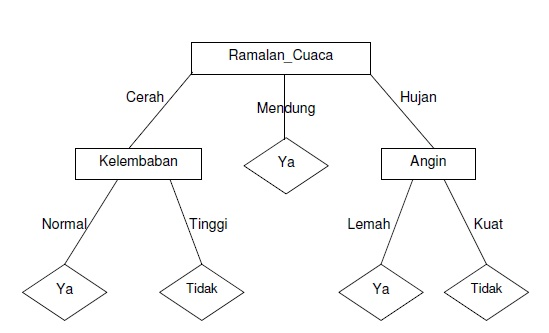
\includegraphics[scale=0.5]{figures/1mrdt.jpg}
\caption{Klasifikasi Binari}
\label{contoh}
\end{figure}
\end{enumerate}


\subsection{ Pengertian Supervised Learning, Unsupervised Learning dan Clustering dan Illustrasi gambar}
\begin{enumerate}
\item Supervised learning adalah sesuatu pembelajaran yang terawasi yang dimana jika output yang diharapkan telah diketahui sebelum-sebelumnya. Biasanya Supervised Learning ini dilakukan dengan menggunakan data yang sudah ada. Pada metode ini, setiap pola yang diberikan kedalam jaringan saraf tiruan setelah diketahui outputnya. Satu pola input akan diberikan ke satu neuron pada lapisan-lapisan input. Pola-pola ini akan dirambatkan di sepanjang jaringan syaraf hingga sampai ke neuron pada lapisan output tersebut. Algoritma pembelajaran yang diawasi menganalisis data pelatihan dan menghasilkan fungsi yang disimpulkan, yang dapat digunakan untuk memetakan contoh-contoh baru. Skenario optimal akan memungkinkan algoritma menentukan label kelas dengan benar untuk instance yang tidak terlihat.
\begin{figure}[ht]
\centering
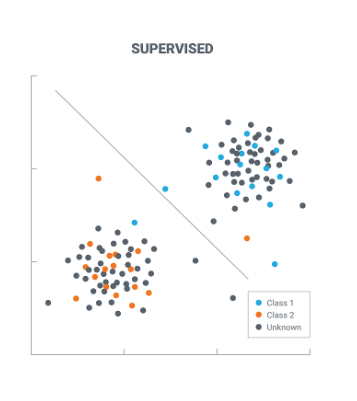
\includegraphics[scale=0.5]{figures/2mrdt.png}
\caption{Supervised Learning}
\label{contoh}
\end{figure}

\item Unsupervised learning merupakan sebuah pembelarajan yang tidak terawasi dimana tidak memerlukan target output. Pada metode ini tidak dapat ditentukan hasil seperti apa yang diharapkan selama proses pembelajaran, nilai bobot yang disusun dalam proses range tertentu tergantung pada sebuah nilai output yang telah diberikan. Tujuan metode unsupervised learning ini agar dapat mengelompokkan unit-unit yang hampir sama dalam satu area tertentu. Pembelajaran ini biasanya sangat cocok untuk klasifikasi pola-pola. Contohny algoritma jaringan saraf tiruan yang menggunakan metode unsupervised ini merupakan competitive, kohonen, LVQ(Learning Vector Quantization), neocognitron.
\begin{figure}[ht]
\centering
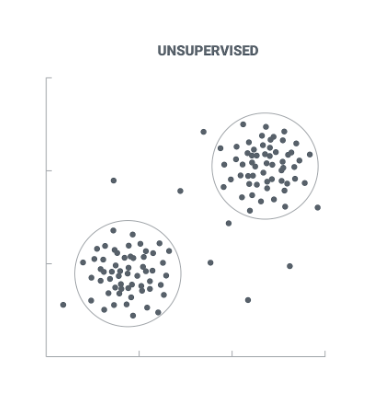
\includegraphics[scale=0.5]{figures/3mrdt.png}
\caption{Unsupervised Learning}
\label{contoh}
\end{figure}
\item Analisis Cluster adalah sebuah teknik statistika yang dapat berguna untuk mengelompokkan sebuah objek-objek ataupun variable-variable ke dalam beberapa grup tertentu dimana pada setiap objek atau variable yang telah terbentuk mempunyai sifat dan karakteristik yang berdekatan tersebut.Gagasan populer mengenai cluster termasuk kelompok dengan jarak kecil antara anggota cluster, area padat ruang data, interval atau distribusi statistik tertentu. Clustering karena itu dapat dirumuskan sebagai masalah optimasi multi-objektif. Algoritma pengelompokan dan pengaturan parameter yang sesuai (termasuk parameter seperti fungsi jarak yang akan digunakan, ambang kepadatan atau jumlah cluster yang diharapkan) tergantung pada set data individual dan penggunaan hasil yang dimaksudkan.
\begin{figure}[ht]
\centering
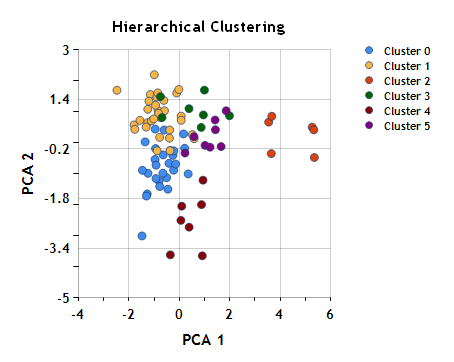
\includegraphics[scale=0.5]{figures/4mrdt.png}
\caption{Cluster}
\label{contoh}
\end{figure}
\end{enumerate}

\subsection{Evaluasi dan akurasi dan Illustrasi gambar}
\begin{enumerate}
\item Evaluasi merupakan suatu langkah bagaimana agar dapat mengevaluasi seberapa baik model bekerja dengan cara mengukur tingkat akurasinya. Dan akurasi tersebut akan didefinisikan menjadi sebuah persentasi studi kasus yang telah diklasifikasikan dengan benar. Dapat juga untuk menganalisis kesalahan yang dibuat oleh sebuah model, atau tingkat kebingungannya, menggunakan matriks kebingungan. Matriks kebingungan mengacu pada sebuah kebingungan dalam model, tetapi matriks kebingungan ini bisa menjadi sedikit sulit untuk dipahami ketika mereka menjadi sangat besar.
\begin{figure}[ht]
\centering
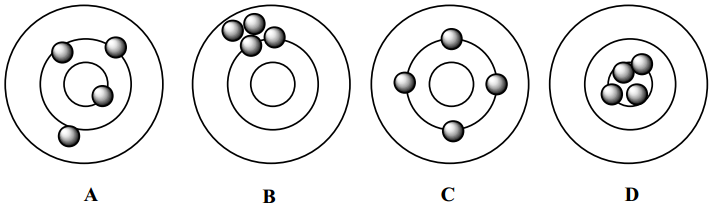
\includegraphics[scale=0.5]{figures/5mrdt.png}
\caption{ Evaluasi dan Akurasi}
\label{contoh}
\end{figure}
\end{enumerate}

\subsection{ Cara membuat dan membaca confusion matrix, buat confusion matrix }
\begin{enumerate}
\item Cara membuat dan membaca confusion matrix :
\begin{itemize}
\item 1)	Menentukan pokok sebuah permasalahan dan atribut-atributnya, misal gaji dan listik.
\item 2)	Buat pohon keputusan
\item 3)	Lalu data testingnya
\item 4)	Lalu mencari nilai a, b, c, dan d. Semisal a = 5, b = 1, c = 1, dan d = 3.
\item 5)	Selanjutnya mencari nilai recall, precision, accuracy, serta dan error rate.
\end{itemize}
\item Berikut adalah contoh dari confusion matrix :
\begin{itemize}
\item Recall =3/(1+3) = 0,75
\item Precision = 3/(1+3) = 0,75
\item Accuracy =(5+3)/(5+1+1+3) = 0,8
\item Error Rate =(1+1)/(5+1+1+3) = 0,2
\end{itemize}
\end{enumerate}

\subsection{Membuat cara K-fold cross validation bekerja dengan gambar ilustrasi}
\begin{enumerate}
\item Cara kerja K-fold cross validation :
\begin{itemize}
\item 1)	Total instance dibagi menjadi N bagian.
\item 2)	Fold yang pertama adalah bagian pertama menjadi data uji (testing data) dan sisanya menjadi training data.
\item 3)	Lalu hitung akurasi berdasarkan porsi data tersebut dengan menggunakan persamaan.
\item 4)	Fold yang ke dua adalah bagian ke dua menjadi data uji (testing data) dan sisanya training data. 
\item 5)	Kemudian hitung akurasi berdasarkan porsi data tersebut.
\item 6)	Dan seterusnya hingga habis mencapai fold ke-K.
\item 7)	Terakhir hitung rata-rata akurasi K buah.
\end{itemize}
\begin{figure}[ht]
\centering
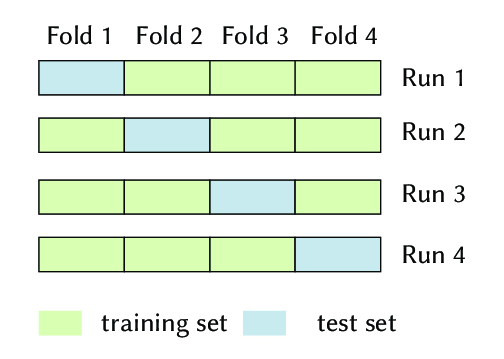
\includegraphics[scale=0.5]{figures/6mrdt.png}
\caption{K-fold cross validation}
\label{contoh}
\end{figure}
\end{enumerate}

\subsection{Decision tree dengan gambar ilustrasi}
\begin{enumerate}
\item Decision Tree dalah metode pembelajaran yang diawasi non-parametrik yang digunakan untuk mengklasifikasi dan regresi. Tujuannya adalah untuk membuat model yang memprediksi nilai variabel target dengan mempelajari aturan keputusan sederhana yang disimpulkan dari fitur data. Decision tree memadukan antara eksplorasi data dan sebuah pemodelan, sehingga sangat bagus sebagai langkah awal dalam proses pemodelan bahkan ketika dijadikan menjadi sebuah model akhir dari beberapa teknik lain.\\
\begin{figure}[ht]
\centering
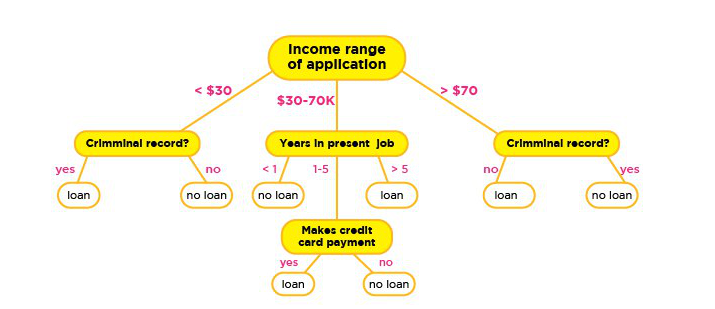
\includegraphics[scale=0.5]{figures/7mrdt.png}
\caption{Decision Tree}
\label{contoh}
\end{figure}
\end{enumerate}

\subsection{Information Gain dan entropi dengan gambar ilustrasi}
\begin{enumerate}
\item Information gain dapat didasarkan kepada penurunan entropi setelah dataset yang sebelumnya dapat dibagi pada atributnya. Untuk membangun sebuah decision tree, merupakan cara agar semua tentang menemukan atribut yang mengembalikan perolehan informasi tertinggi dari yang lainnya.
\begin{figure}[ht]
\centering
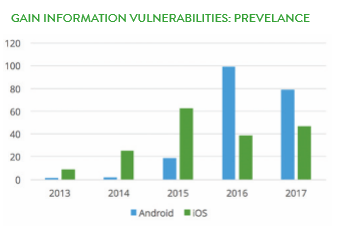
\includegraphics[scale=0.5]{figures/8mrdt.png}
\caption{Information gain}
\label{contoh}
\end{figure}
\item Entropi adalah cara untuk mengukur keacakan dalam sebuah sistem informasi yang sedang diproses. Semakin tinggi entropi, mka hasilnya semakin sulit untuk menarik kesimpulan dari informasi tersebut. Melempar koin merupakan salah satu contoh tindakan yang memberikan informasi yang random. Untuk koin yang tidak memiliki afinitas untuk kepala atau ekor, hasil dari sejumlah lemparan sulit diprediksi. Mengapa? Karena tidak ada hubungan antara membalik dan hasilnya. Inilah inti dari entropi.
\begin{figure}[ht]
\centering
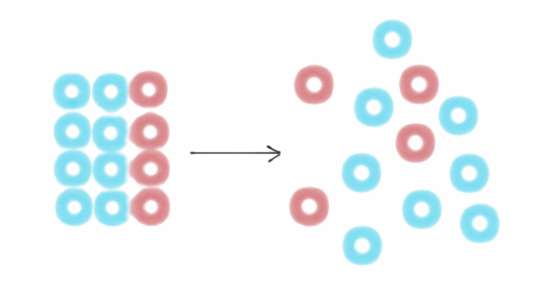
\includegraphics[scale=0.5]{figures/9mrdt.png}
\caption{Entropi}
\label{contoh}
\end{figure}
\end{enumerate}

 